\section{System Design and Implementation} \label{systemdesign_and_implementation}

Current cloud management platforms make simplified assumptions about the hardware in the datacentre and its usage. Hardware is by default powerful rack or blade servers, they are virtualised, and always on. Thus cloud management platforms on the market are suboptimal for certain use cases.

HPC and Big Data applications require highly optimised and powerful hardware. In such applications, the overheads imposed by virtualisation are undesirable and for maximum efficiency the cluster should consist of bare-metal computing nodes. Furthermore other advantages of virtualisation such as multi-tenancy and scaling are not useful in bare-metal computing.

On the other end of the spectrum are very weak computers with limited computing power, memory, I/O throughput and storage. These machines can be a worthwhile addition to a cloud environment for running small low intensity tasks: They are significantly cheaper to traditional datacentre hardware costing some hundred Euros per machine instead of thousands like a single rack server. They do not require much space to store, use less electricity and output less heat. Virtualisation may not be applicable for such machines either due to hardware not supporting virtualisation in the first place, or as the virtualisation overhead may consume large enough share of a machine's resources rendering it incapable to perform or at least severely restricting any other functionality besides virtualisation. With low end computers virtualisation benefits like multi-tenancy and running multiple operating systems in parallel may simply not be possible because of limited capabilities. Using these machines in a heterogeneous cluster requires treating them like a traditional bare-metal nodes, albeit not nearly as powerful.

In order to leverage on bare-metal nodes in a heterogeneous and possibly even in a hybrid cloud, the task schedulers require a view to the underlying infrastructure so that they can allocate tasks to nodes fitted to perform them. To extend the usage to befit hybrid clouds in addition to heterogeneous, the orchestrator has to be vendor agnostic too. This thesis presents prototype extensions to Cloudify's \cite{cloudify} client agents, which are used to communicate between the nodes and Cloudify Manager. Extensions are going to allow two things:

\begin{enumerate}
\item \textit{Allow the Manager to gain information about the nodes' hardware capabilities, a feature that is currently lacking from the project.}
\item \textit{Enable node discovery in the cluster.}
\end{enumerate}

Currently managing the composition of the host-pool is a manual effort. The hosts nodes in the cluster can either be configured before launching the cluster using a host pool YAML file or with REST API calls. Therefore monitoring for failing nodes and adding new ones, especially en masse, is an arduous task. A discovery mechanism for new nodes in the cluster would ameliorate if not solve the problem, even if replacing faulty hardware is more often than not a manual task. Additionally discovery mechanism would allow \textit{Bring-your-own-host} kind of functionality.

 \subsection{Design overview}
 
Centrepiece in Cloudify's architecture for achieving the set goals for more detailed information and node discovery is the \textit{Host-pool service} \cite{host-pool-service}. Host-pool service is a RESTful service to which Cloudify Manager can make calls via Host-pool plugin to gain information about nodes that compose the cluster. It can also allocate hosts for jobs run by the manager as well as deallocate them. One major feature host-pool service provides is adding hosts to the pool during runtime. It can also remove hosts from the pool and both operations are performed with a similar REST API call. A Cloudify set-up without host-pool service can not make use of generic cluster comprising of different bare-metal nodes. The relationships between different Cloudify components are illustrated in figure ~\ref{fig:cloudify_roles}.
 
 \begin{figure}[ht!]
\centering
  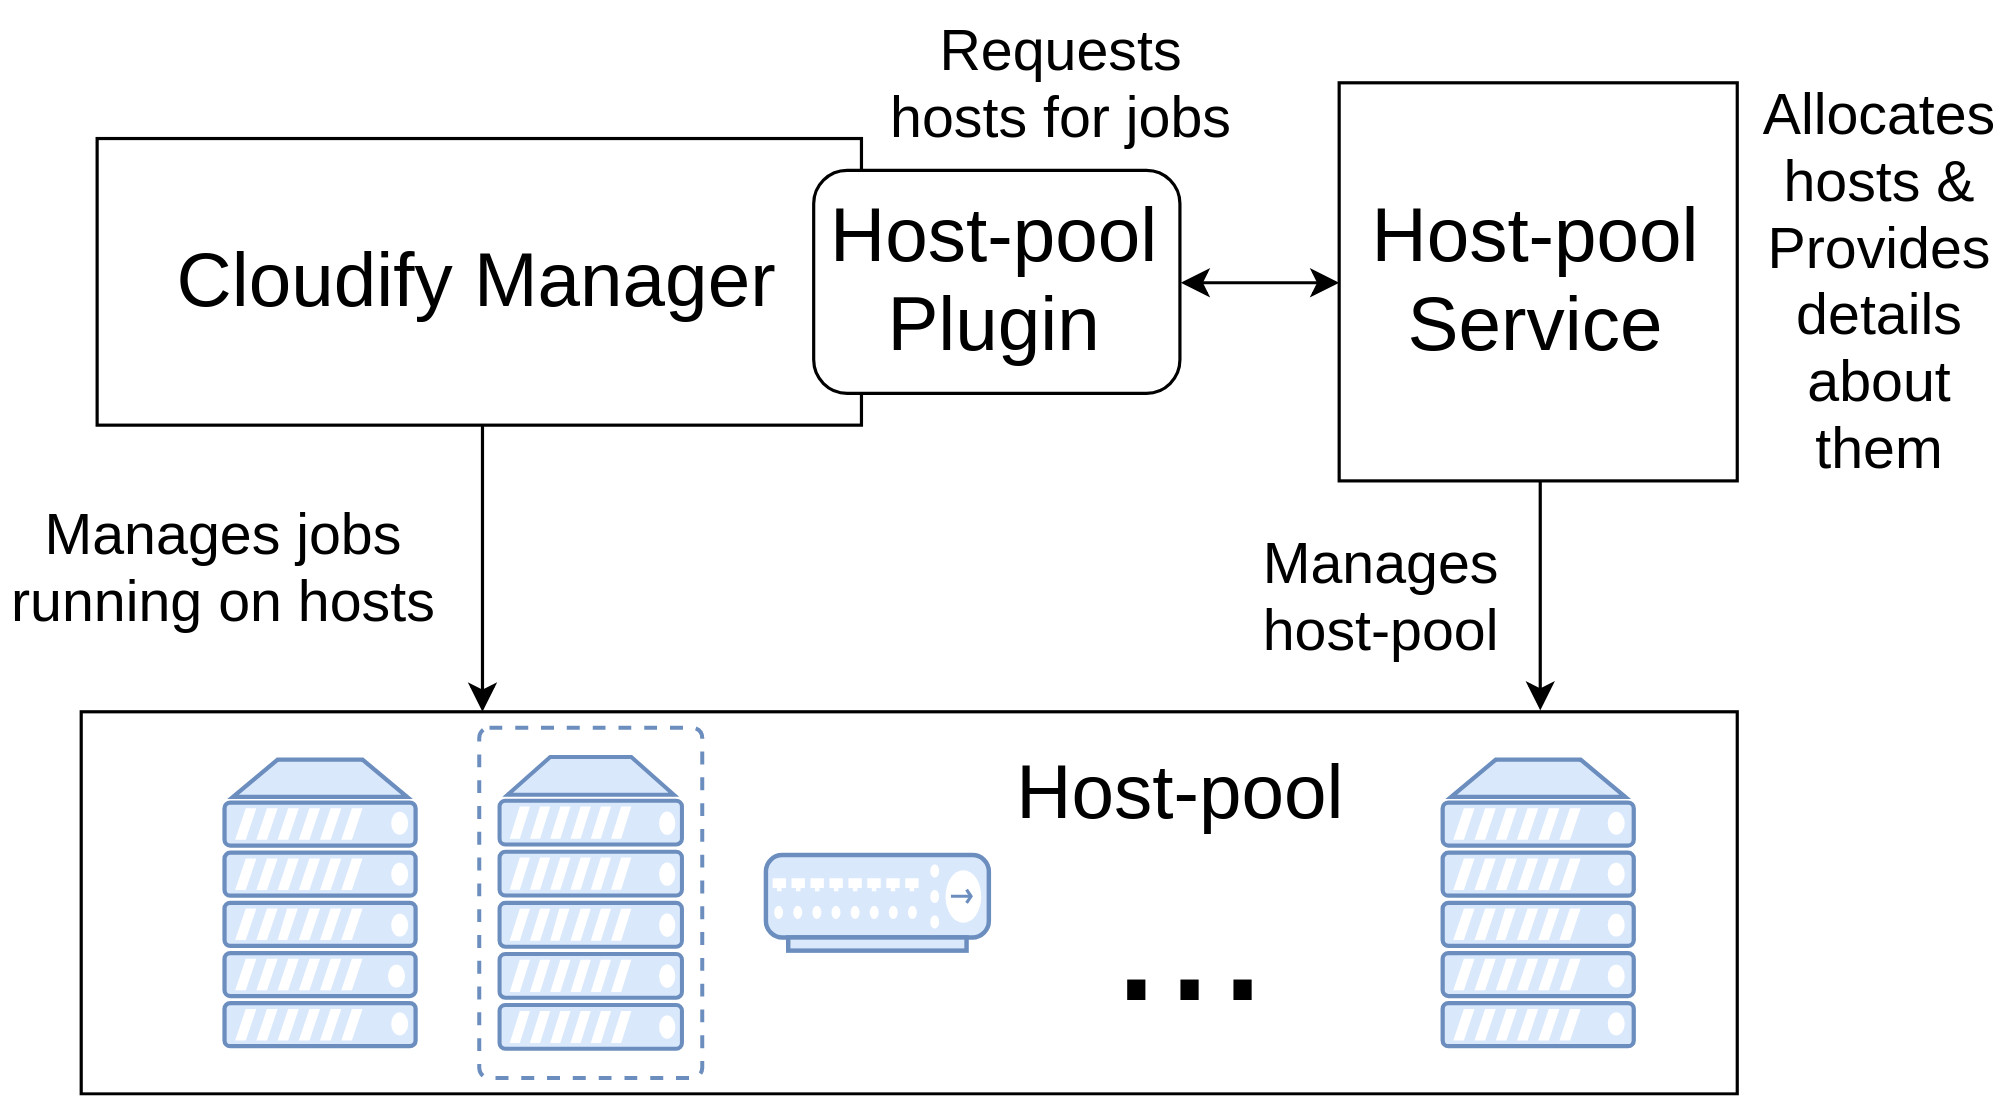
\includegraphics[width=\textwidth, keepaspectratio]{Cloudify_roles.png}%
  \caption{The role of the Host-Pool Service.}
  \label{fig:cloudify_roles}
\end{figure}

The goal for retrieving more hardware information from hosts requires running a script on the hosts. Currently the information host-pool service provides is concise, providing information like the operating system of the host, available endpoints and login credentials. It does not in fact query the host themselves. In order to get any performance information, host-pool service should run a script querying for the hardware data and storing the results when adding the host to the logical pool. This requires extending  the host-pool service.

The goal for host discovery and automated host pool management will be implemented as an additional Discovery Service.
The role of the Discovery service is twofold as seen on figure ~\ref{fig:discovery_service}.


\begin{figure}[ht!]
\centering
  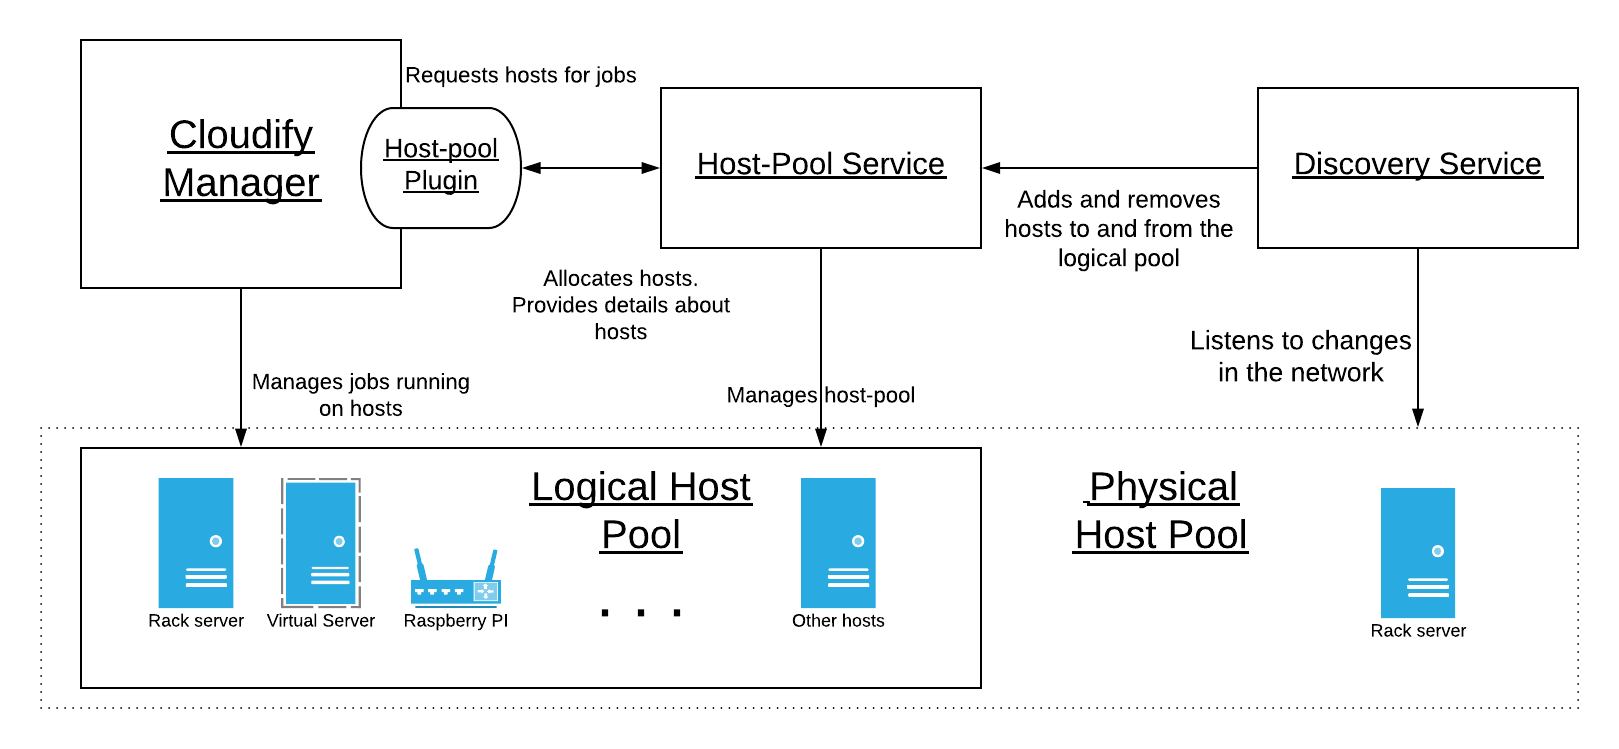
\includegraphics[width=\textwidth, keepaspectratio]{Discovery_service.png}%
  \caption{Discovery service's relation to other Cloudify Components.}
  \label{fig:discovery_service}
\end{figure}

The Discovery Service constantly monitors the network and its devices and keeps track of discovered devices and their health. When a new device is detected in the network its details are added to Discovery Service's local memory and a REST API call to add the device to the logical pool of hosts is made to Host-pool Service. Device health is monitored periodically and after a set number of failed health checks are detected, the device is removed from Discovery Service's memory and a REST API call to remove the host from the logical pool is made.